\subsection{The Challenges of Monitoring}
Consider the following examples of automated tasks that might be found in one of three different application domains:
\begin{enumerate}
\item An automated stock market trading system monitors the distribution of buy and sell orders of a particular stock to identify the best time and price for its own orders.
\item A corporate data warehouse monitors the current status of its production facilities, warehoused inventory and active demand for its products in order to preemptively identify supply chain problems.
\item A compute cluster monitors its current status overnight to alert a network administrator when some of its hardware fails, but only if a distributed task running on the cluster is at risk of becoming unavailable.
\end{enumerate}

These are only a few examples of application domains where automated realtime {\em monitoring} systems are necessary.  Monitoring plays a prominent role in a broad range of domains including regulatory compliance\cite{basel2}, fraud detection\cite{ibmfico}, advertising\cite{agarwal2010forecasting}, big-data science\cite{hey2009fourth}, disaster prediction\cite{scholz1973earthquake}, machine learning\cite{olesen2008real}, and many more.  Unfortunately, although many commonalities exist between these domains, automated monitoring systems are still implemented entirely by hand on a per-domain basis.

Fundamentally, automated monitoring is a data-management challenge.  Even for the relatively simple conditions from the three examples above, rapid changes to the state of the world can easily overwhelm a naively implemented monitoring system.  Filtering, projection, and aggregation -- the traditional tools of the database community -- are all necessary to reduce the data to manageable levels.  

However, simple data manipulation is not sufficient.  In order to achieve realtime performance, automated monitoring systems must exploit the incrementality of their application domain.  As servers go down in the compute cluster example, an intelligently designed monitoring application will not attempt to recompute the availability of each task from scratch.  Rather, the application will maintain a running tally of how many ``up'' servers are assigned to each task and adjust the tally as servers come up or go down.  

Although this sort of incrementality is often obvious to a human developer, techniques for automatic identification and exploitation of such patterns have not been developed within the database community.  Active database \cite{morgenstern1983active} and complex stream event processing (CEP)\cite{?} techniques both address the challenges of monitoring persistent state, yet neither approach fully identifies or exploits incrementality.

As we will now show through experimental (and some anecdotal) evidence, the state of the art techniques of the database community: both active databases and CEP are ill suited for the task of building automated monitoring systems.

We consider the three example scenarios as described above.  Each monitoring task is implemented using triggers in Postgres and two commercial database systems, and using CEP in two commercial stream processing systems\footnote{The names of the commercial databases and stream processors are kept anonymous due to restrictions in their license agreements.}.  Concretely, the scenarios are as follows:

\begin{figure}
\tinysection{Example \ref{ex:dbfail:stock}}
\begin{verbatim}
-- Example 2.1 --
CREATE TABLE bids(volume float, price float);
CREATE TABLE asks(volume float, price float);
\end{verbatim}

\tinysection{Example \ref{ex:dbfail:tpch}}'s schema is identical to the TPC-H schema\cite{tpch}.

\tinysection{Example \ref{ex:dbfail:network}}
\begin{verbatim}
CREATE TABLE Server(ssid int, status int);
CREATE TABLE Task(ttid int, priority int);
CREATE TABLE Assignment(asid int, atid int);
\end{verbatim}

\label{fig:dbfail:schemas}
\caption{Schemas for the three example scenarios}
\end{figure}

\begin{example}
\label{ex:dbfail:stock}
A stock market trading system monitors the spread across significant orders for a particular stock (i.e., orders larger than 0.01\% of the total volume of orders for the stock).  Given the table schemas defined in Figure \ref{fig:dbfail:schemas}, we are interested in monitoring the value represented by the result of the following SQL query:
% test/sql/finance/pricespread.sql
\begin{verbatim}
SELECT SUM(a.price - b.price)
FROM   bids b, asks a
WHERE  b.volume > 0.0001 * (SELECT SUM(b1.volume) 
                            FROM   bids b1)
  AND  a.volume > 0.0001 * (SELECT SUM(a1.volume) 
                            FROM   asks a1);
\end{verbatim}

\end{example}

\begin{example}
\label{ex:dbfail:tpch}
A corporate data warehouse monitors the volume of of parts of each type being shipped between each region based on the locations of the supplier and the client.  Given the standard TPC-H benchmark schema\cite{counciltpc}, we can express this monitoring task as the following SQL group-by query: 
% test/sql/tpch/ssb4.sql
\begin{verbatim}
SELECT   sn.regionkey, cn.regionkey,
         p.type, SUM(li.quantity)
FROM     CUSTOMER c, ORDERS o, LINEITEM li, PART p, 
         SUPPLIER s, NATION cn, NATION sn
WHERE       c.custkey = o.custkey
  AND      o.orderkey = li.orderkey
  AND       p.partkey = li.partkey
  AND       s.suppkey = li.suppkey
  AND    cn.nationkey = c.nationkey
  AND    sn.nationkey = s.nationkey
GROUP BY sn.regionkey, cn.regionkey, PART.type;
\end{verbatim}

\end{example}

\begin{example}
\label{ex:dbfail:network}
A cluster monitoring system keeps monitors servers assigned to work on different compute tasks -- the system issues an alert whenever the number of failed servers assigned to a given task exceeds a given threshold (e.g., 50\%).  These alerts are dispatched based on priority, and number of threatened tasks.  Given the table schemas defined in Figure \ref{fig:dbfail:schemas}, we can represent this monitoring task as monitoring the result of the following SQL group-by query (e.g., triggering an alert whenever the query returns a non-empty result):
% test/sql/clusteravailable_priority.sql
\begin{verbatim}
SELECT priority, COUNT(*)
FROM   Task t
WHERE  (SELECT COUNT(*) 
        FROM Assignment a2,Server s2
        WHERE t.ttid = a2.atid 
        AND a2.asid = s2.ssid) * 0.5 > 
       (SELECT COUNT(*) 
        FROM Assignment a3,Server s3
        WHERE t.ttid = a3.atid 
        AND a3.asid = s3.ssid 
        AND s3.status = 1)
GROUP BY t.priority;
\end{verbatim}

\end{example}

\subsection{Monitoring with Active Databases}
\label{sec:dbfail:active}
Of the two monitoring technologies considered to be state-of-the-art in the database community, we first consider {\em Active Databases}\cite{morgenstern1983active} -- systems where derived and non-derived (base) data are all-but indistinguishable.  As noted in the initial description of the idea, monitoring in such a system is easy from the user's perspective; The user need only declare how the value to be monitored is derived.  

Unfortunately, production-quality implementations of this idea have not been able to fully realize its possibilities.  Both the declarative rules of \cite{morgenstern1983active}, and the equivalent notion of on-conditions\cite{taylor1976codasyl} or {\em triggers}\cite{mccarthy1989architecture} are designed to be restrictive in order to limit the amount of computation effected by an update to the base data.  Although simple declarative rules or triggers can be combined into more complex conditions\cite{DBLP:conf/icde/ZimmerU99}, in doing so, users are forced to explicitly specify the implementation strategy.  The benefits of a declarative specification are lost.  Nevertheless, support for triggers can be found in a variety of noncommercial\cite{stonebraker1991postgres,mysql1mysql} and commercial\cite{oracle,graymicrosoft,gassner1993query} database engines.

Efforts to identify incrementality in declaratively specified monitoring tasks can be found in work on {\em incremental view maintenance} (IVM)\cite{gupta1993maintaining,ceri1991deriving}.  Monitoring tasks are specified as declarative SQL queries -- the result of the query is kept materialized in the database at all times.  When the base data changes, the IVM system does not recompute the monitored query from scratch.  Rather, it evaluates a delta query -- derived automatically from the monitored query -- the result of which indicates how the monitored query's result is affected by the change to the base data.

\begin{example}
For example, consider the query from Example \ref{ex:dbfail:tpch} and an insertion into the {\tt LINEITEM} table:
\begin{verbatim}
INSERT INTO 
LINEITEM(orderkey, partkey, suppkey, quantity)
VALUES  (37,       42,      7,       100);
\end{verbatim}

We can run the following (delta) query:
\begin{verbatim}
SELECT   sn.regionkey, cn.regionkey,
         p.type, SUM(100) 
FROM     CUSTOMER c, ORDERS o, PART p, 
         SUPPLIER s, NATION cn, NATION sn
WHERE       c.custkey = o.custkey
  AND      o.orderkey = 37
  AND       p.partkey = 42
  AND       s.suppkey = 7
  AND    cn.nationkey = c.nationkey
  AND    sn.nationkey = s.nationkey
GROUP BY sn.regionkey, cn.regionkey, PART.type;
\end{verbatim}

Note that all columns from the {\tt LINEITEM} table have been replaced by the corresponding value from the inserted tuple.  

The tuples resulting from running this query represent how the monitored query changes.  We can merge the new results with the old ones by adding the sum columns of the delta query and old results for tuples with identical group-by columns (treating non-existent rows as having an effective sum value of 0).

After merging it with the delta, the materialized view correctly represents the results of the original query after the insertion into {\tt LINEITEM}.
\end{example}

Because the delta query is simpler, it can be evaluated more efficiently than the original, conceivably saving time on updates.  IVM functionality has been implemented into most commercial database systems, including the two we test.

\begin{figure*}
\begin{center}
\begin{tabular}{ccc}
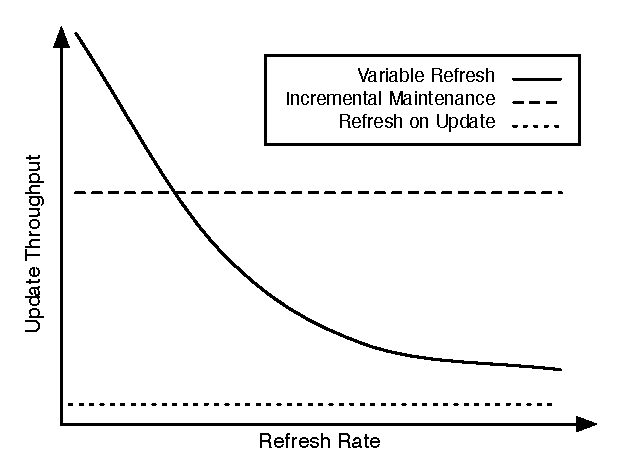
\includegraphics[width=2in]{../graphics-tmp/placeholder_db_result} &
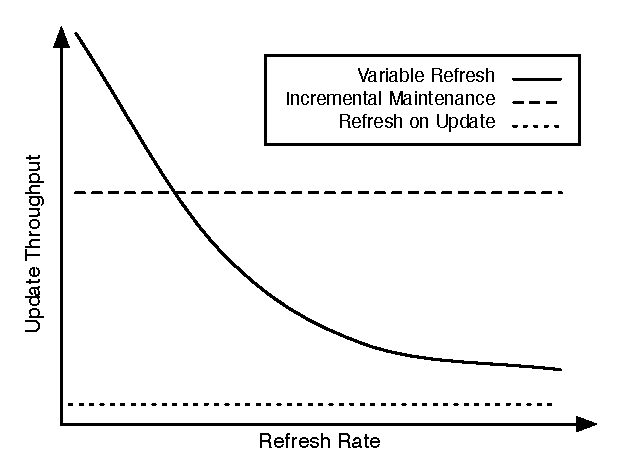
\includegraphics[width=2in]{../graphics-tmp/placeholder_db_result} &
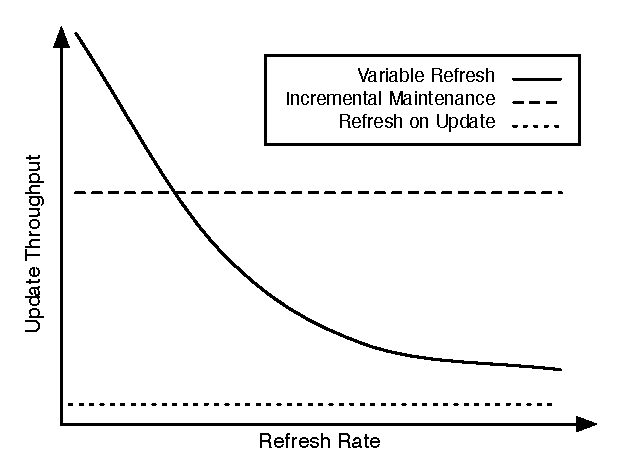
\includegraphics[width=2in]{../graphics-tmp/placeholder_db_result} \\
(a) & (b) & (c)
\end{tabular}
\end{center}
\label{fig:dbfail:postgres}
\caption{Performance results for Postgres on Examples \ref{ex:dbfail:stock} (a), \ref{ex:dbfail:tpch} (b), and \ref{ex:dbfail:network} (c).}
\end{figure*}
\begin{figure*}
\begin{center}
\begin{tabular}{ccc}
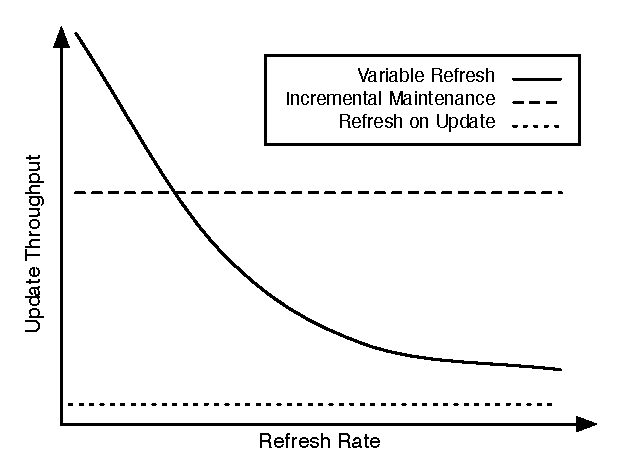
\includegraphics[width=2in]{../graphics-tmp/placeholder_db_result} &
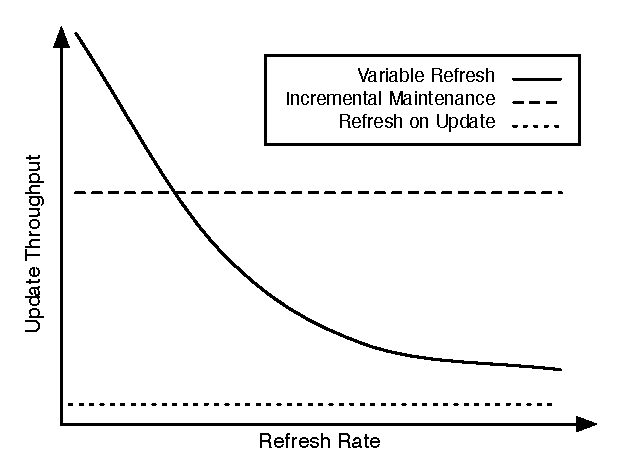
\includegraphics[width=2in]{../graphics-tmp/placeholder_db_result} &
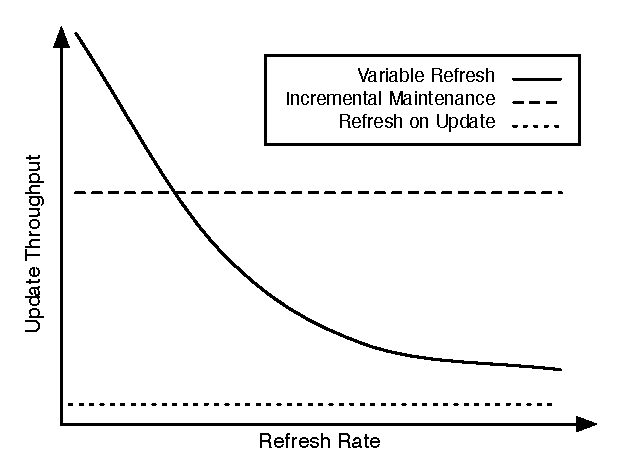
\includegraphics[width=2in]{../graphics-tmp/placeholder_db_result} \\
(a) & (b) & (c)
\end{tabular}
\end{center}
\label{fig:dbfail:CD1}
\caption{Performance results for Commercial DBMS 1 on Examples \ref{ex:dbfail:stock} (a), \ref{ex:dbfail:tpch} (b), and \ref{ex:dbfail:network} (c).}
\end{figure*}\begin{figure*}
\begin{center}
\begin{tabular}{ccc}
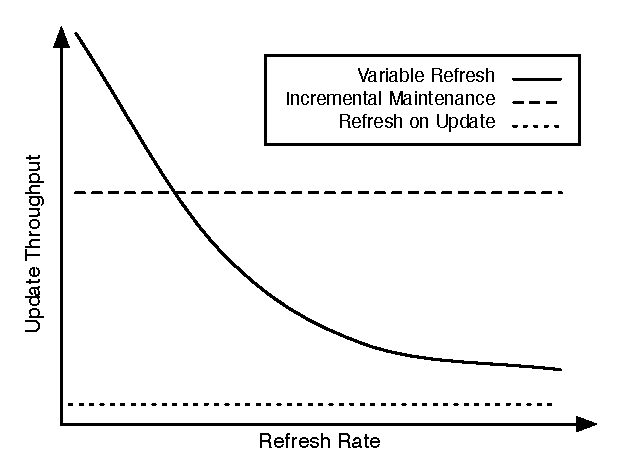
\includegraphics[width=2in]{../graphics-tmp/placeholder_db_result} &
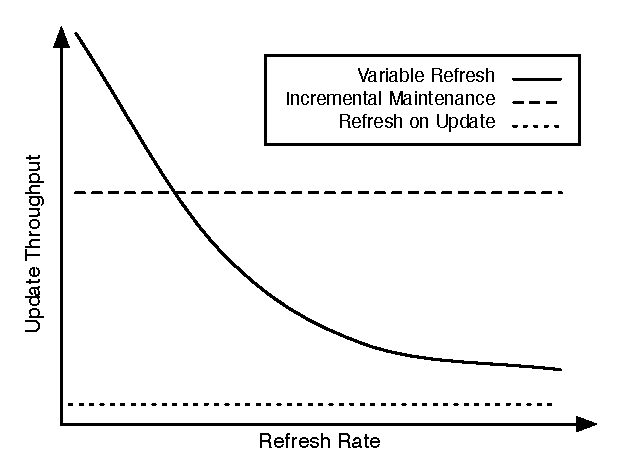
\includegraphics[width=2in]{../graphics-tmp/placeholder_db_result} &
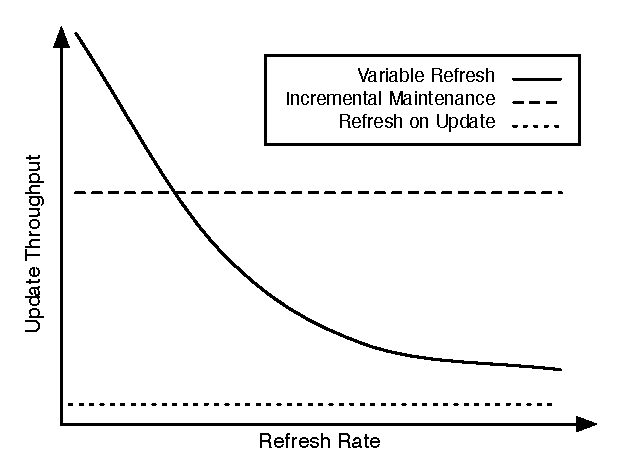
\includegraphics[width=2in]{../graphics-tmp/placeholder_db_result} \\
(a) & (b) & (c)
\end{tabular}
\end{center}
\label{fig:dbfail:CD2}
\caption{Performance results for Commercial DBMS 2 on Examples \ref{ex:dbfail:stock} (a), \ref{ex:dbfail:tpch} (b), and \ref{ex:dbfail:network} (c).}
\end{figure*}

Figures \ref{fig:dbfail:postgres}, \ref{fig:dbfail:CD1}, and \ref{fig:dbfail:CD2} show how the Postgres and two Commercial DBMSes (respectively) perform in each of the three example scenarios.  We consider three techniques for keeping a live view of the query result:
\begin{itemize}
\item {\bf Variable Refresh:} Periodically re-evaluate the query.  Note that in this implementation this results in the query not being monitored continually; The implementation can not detect trigger conditions which arise and disappear in between re-evaluations.
\item {\bf Full Refresh:} Use triggers to initiate a full refresh of the query results after every update to a base relation.  
\item {\bf Incremental Maintenance:} Use IVM to update the query results after every update to the base relation.  In the case of Postgres where IVM is not natively supported, we compute the delta query by hand and implement it via triggers.
\end{itemize}

\todo{Hardware overview goes here}.  Each graph shows the rate of updates supported by our configuration with respect to the frequency with which the query results are refreshed.  The Full Refresh and Incremental Maintenance implementations refresh the query results after every update, and are unaffected by the desired refresh rate.

\todo{Rewrite this paragraph after we have results}
Even with IVM techniques (which must be implemented by hand for Postgres), these systems can handle a maximum of \todo{fill in} updates per second to the base relations.  If users are willing resort to sampling as infrequently as once per one or ten seconds, it is possible to improve that to as much as \todo{fill in} or \todo{fill in} updates per second respectively.  Even with sampling, this is not sufficient to achieve the sorts of update rates required by our example applications.

\subsection{Monitoring with Stream Processors}
Section \ref{sec:dbfail:active} is perhaps a little unfair.  Although these systems are designed to efficiently process complex queries, even those that support incremental view maintenance are not designed to support rapidly changing data.  Rapidly changing data is the domain of stream processing systems \cite{abadi2003aurora,arvind2003stream,chandrasekaran2003telegraphcq,abadi2005design}.  In a Stream Processing system, users define pipelines similar to traditional query plans, except that each edge in the plan is a continuous stream of data.  Selection and projection operators are evaluated immediately.  Sliding Window Operators\cite{datar2002maintaining} {\em temporarily} store tuples appearing on a stream, and allow joins over the most recent set of tuples.  

Although sliding window operators make it easier for a stream processor to provide realtime performance guarantees, relying exclusively on the sliding window operator precludes the use of persistent state.  Recently, most commercial stream processing systems have added support for hybrid queries over both streaming and static data -- an approach commonly referred to as Complex Event Processing (CEP)\cite{DBLP:conf/sigmod/WuDR06}.   

\begin{figure*}
\begin{center}
\begin{tabular}{ccc}
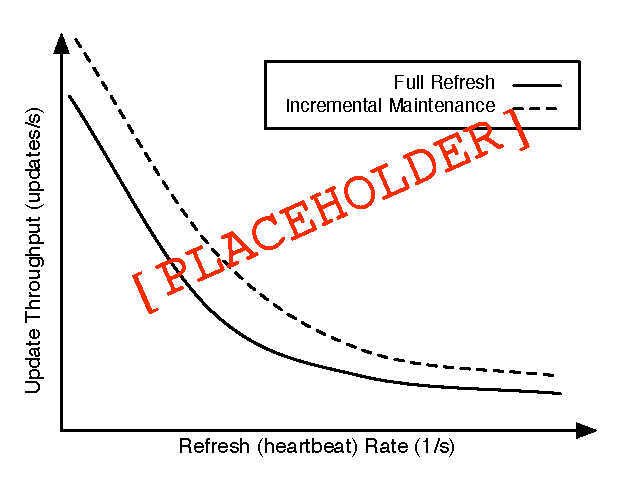
\includegraphics[width=2in]{../graphics-tmp/placeholder_stream_result} &
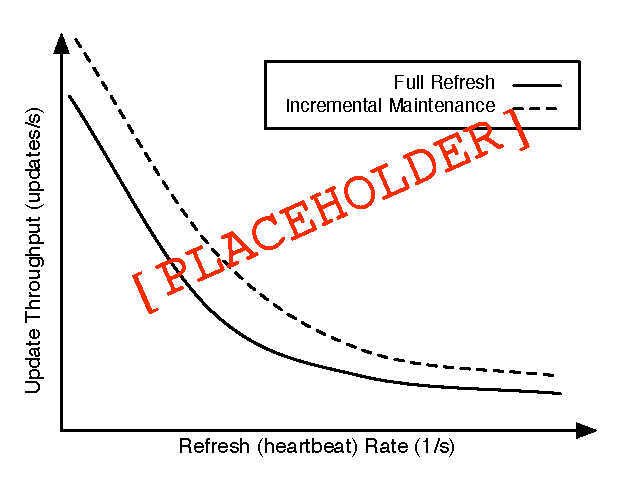
\includegraphics[width=2in]{../graphics-tmp/placeholder_stream_result} &
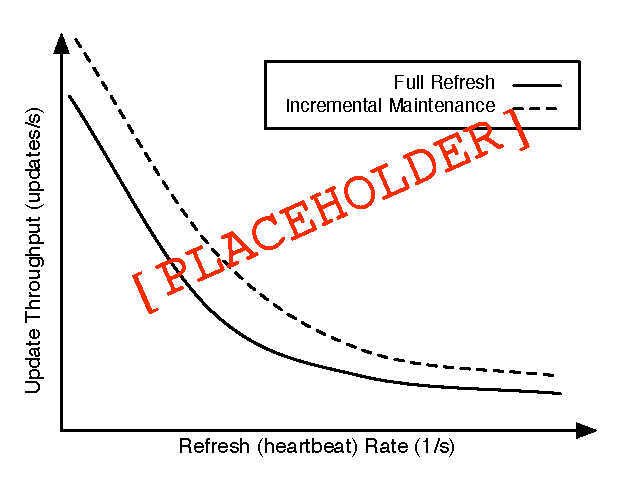
\includegraphics[width=2in]{../graphics-tmp/placeholder_stream_result} \\
(a) & (b) & (c)
\end{tabular}
\end{center}
\label{fig:dbfail:CSP1}
\caption{Performance results for Commercial Stream Processor 1 on Examples \ref{ex:dbfail:stock} (a), \ref{ex:dbfail:tpch} (b), and \ref{ex:dbfail:network} (c).}
\end{figure*}\begin{figure*}
\begin{center}
\begin{tabular}{ccc}
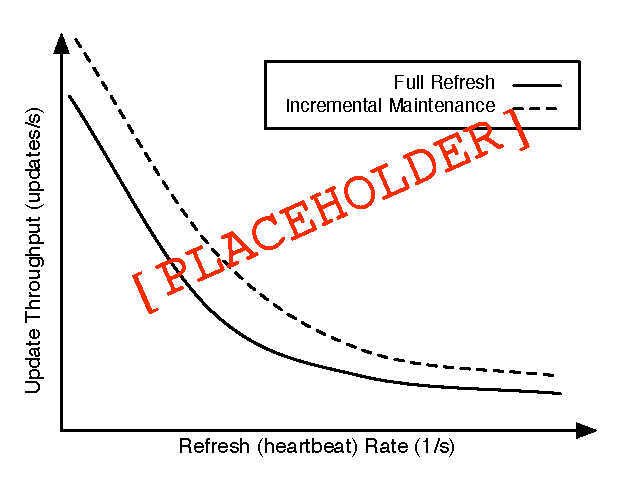
\includegraphics[width=2in]{../graphics-tmp/placeholder_stream_result} &
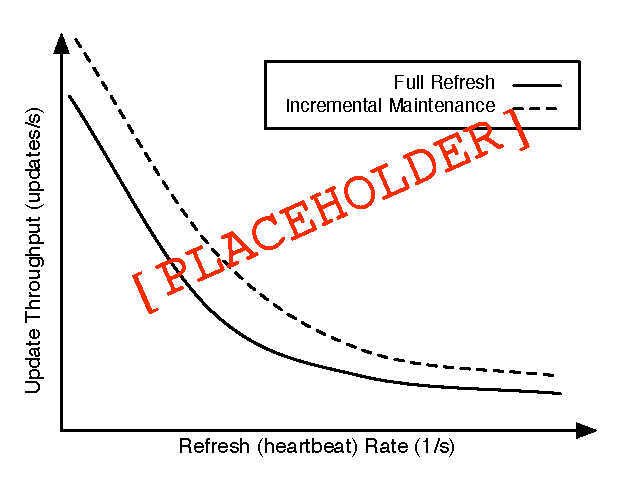
\includegraphics[width=2in]{../graphics-tmp/placeholder_stream_result} &
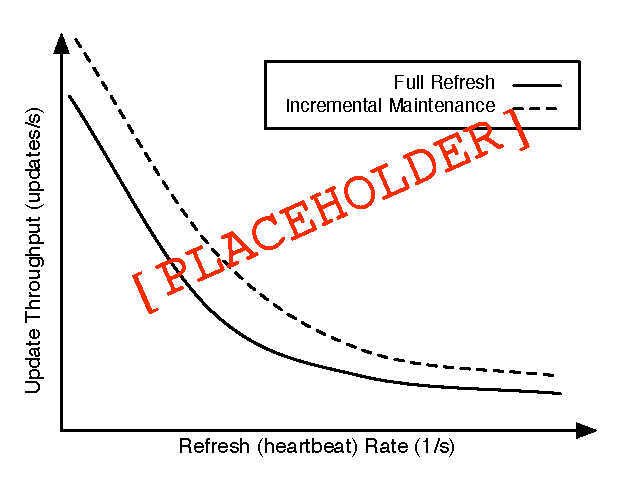
\includegraphics[width=2in]{../graphics-tmp/placeholder_stream_result} \\
(a) & (b) & (c)
\end{tabular}
\end{center}
\label{fig:dbfail:CSP2}
\caption{Performance results for Commercial Stream Processor 2 on Examples \ref{ex:dbfail:stock} (a), \ref{ex:dbfail:tpch} (b), and \ref{ex:dbfail:network} (c).}
\end{figure*}

Figures \ref{fig:dbfail:CSP1}, \ref{fig:dbfail:CSP2}, and \ref{fig:dbfail:CD2} show how two Commercial Stream Processing Systems perform in each of the three example scenarios.  We have also considered a third system, but were unable to implement these scenarios using it.

We consider two implementations of each example in each stream processor: one based on a straight translation of the query into the stream processor's language (Full Refresh), and one based on a translation of the delta queries that would have been generated by IVM (Incremental Maintenance) -- the delta queries are constructed by hand.

\todo{Rewrite this paragraph after we have results}
Even with IVM techniques (which must be implemented by hand in some implementations), these systems can handle a maximum of \todo{fill in} updates per second to the base relations.  This is, in part, the result of a need to lock the base relations before applying updates.  The CEP implementation in the stream processing systems we have analyzed is geared towards implementing tables as purely input or output sources -- persistent state used by the query is assumed to be relatively stable.  

\begin{figure}
\begin{center}
\begin{tabular}{|l|c|c|c|}
\hline
{\bf Engine}   & {\bf 2.1} & {\bf 2.2} & {\bf 2.3} \\\hline
{\bf Postgres} & 8 / 30    & 30 / 120  & 15 / 100 \\\hline
{\bf CDBMS 1}  & 8 / 9     & 30 / 31   & 15 / 16  \\\hline
{\bf CDBMS 2}  & 8 / 9     & 30 / 31   & 15 / 16  \\\hline
{\bf CSP 1}    & 40 / 120  & 60 / 200  & 50 / 200 \\\hline
{\bf CSP 2}    & 40 / 120  & 60 / 200  & 50 / 200 \\\hline
\end{tabular}

\todo{Update these numbers to be correct}
\end{center}
\label{fig:dbfail:locBakeoff}
\caption{Lines of code required to implement each of the example scenarios (including schema definitions) in Postgres, the two commercial database systems (CDBMS 1,2), and the two commercial stream processors (CSP 1,2).  For each engine/scenario pair, both the number of lines to implement the query and it's IVM equivalent are shown (respectively).}
\end{figure}

Another metric that must be considered is implementation complexity.  Figure \ref{fig:dbfail:locBakeoff} shows the number of lines of code required to implement each query in each of these engines.  The use of persistent state in the commercial stream processor forces the user to explicitly manage several messy aspects of the computation (e.g., locking the tables before updating/reading them).  Furthermore, when implementing IVM in systems that do not support it (Postgres and the two stream processors), the delta queries must be computed by hand and explicitly defined, causing a further blowup in number of lines.

\subsection{Implementation Challenges}
\todo{Yanif's horror stories}

\subsection{Other Related Work}